\chapter{Teste na Bancada do Sistema Real} \label{secao:teste_sistema}

Para emular a iluminação solar foram utilizados quatro LEDs de alta potência (\SI{100}{\watt} cada), sendo que a potência fornecida para os LEDs foi controlada de forma a seguir a curva obtida com o modelo citado no capítulo \ref{secao:simulacao_sistema}.

A carga do sistema foi dividida em duas partes: o aquecimento das baterias foi emulado com resistores conectados a saída de um conversor DC-DC. Foram usados três resistores de \SI{10}{\ohm} e um de \SI{47}{\ohm} em paralelo para se obter uma potência próxima a calculada. O resto da curva foi emulado através de uma fonte de quatro quadrantes operando com tensão positiva e corrente negativa.

Duas baterias li-ion ICR18650-30A foram usadas para armazenar energia e 3 paineis solares com 4 conjuntos em paralelo de 10 células KXOB22-12X1F em série foram usados para fornecer a energia.

A bancada utilizada pode ser vista na Figura \ref{figura_bancada_teste}.

\begin{figure}[!htpb]
\begin{center}
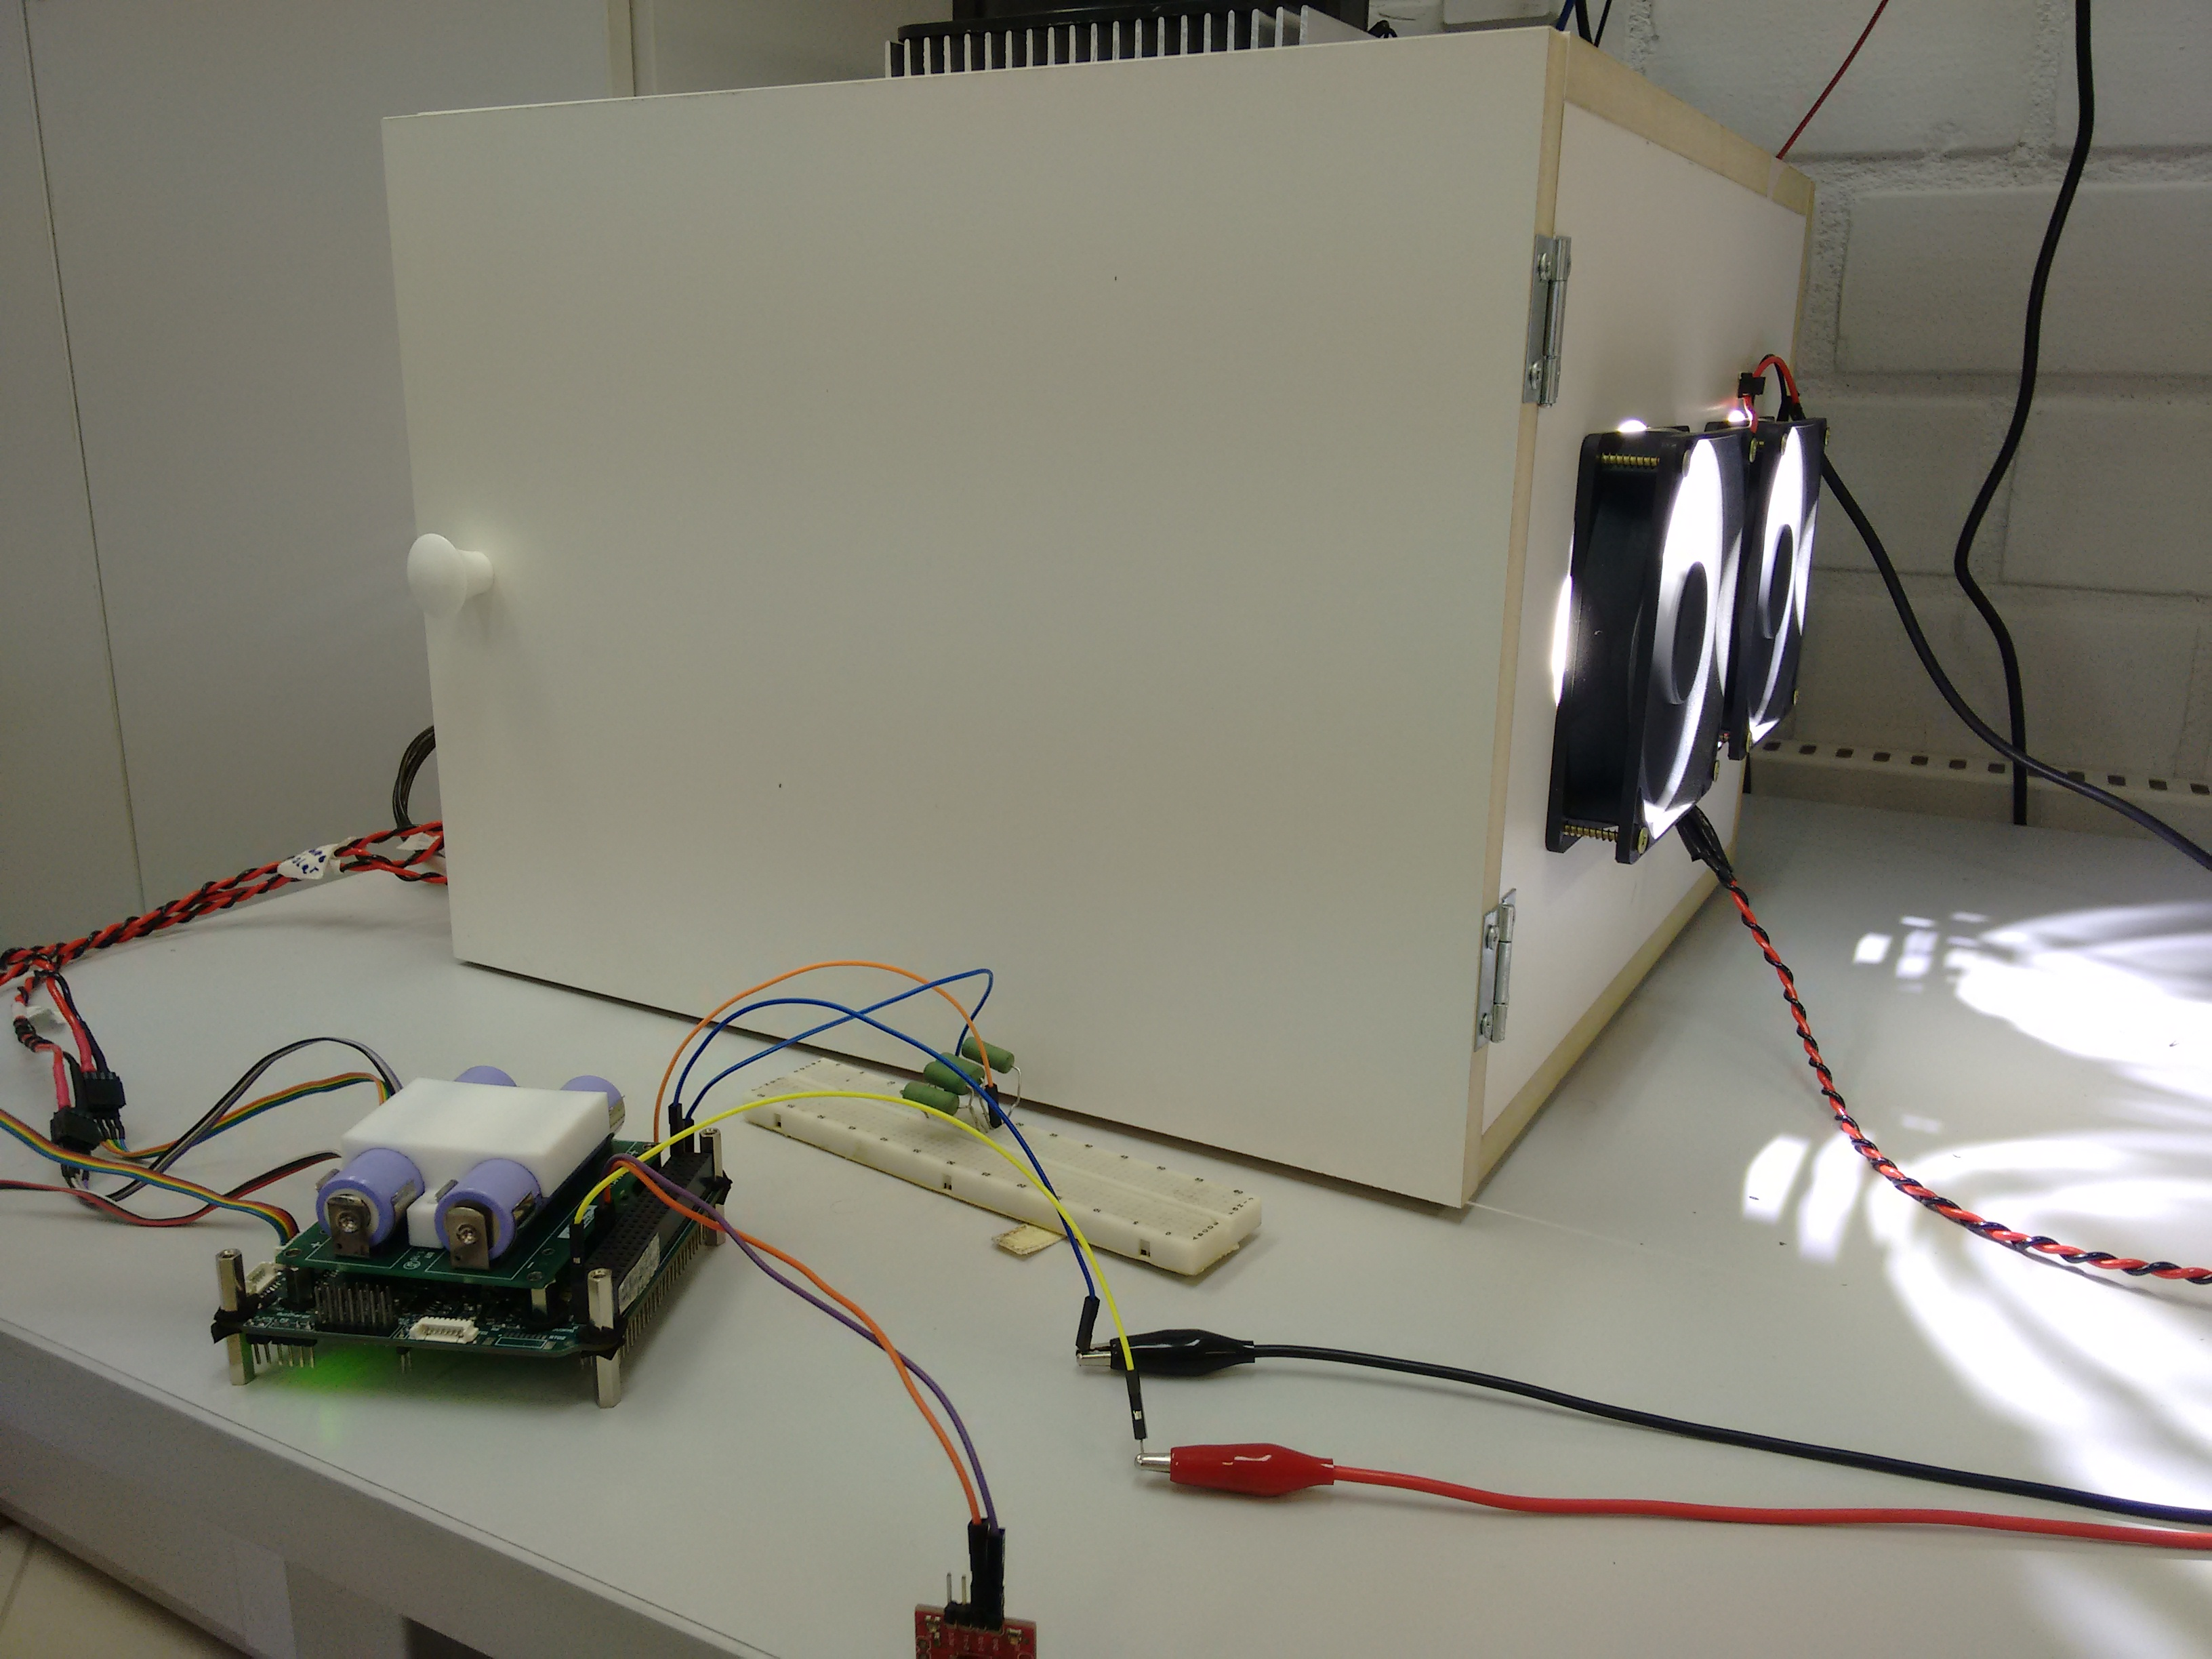
\includegraphics[scale=0.05]{figures/bancada.jpg}
\caption{Bancada de Testes}
\label{figura_bancada_teste}
\end{center}
\end{figure}

As correntes dos painéis estão nas figuras \ref{figura_teste_corrente_painel1}, \ref{figura_teste_corrente_painel2} e \ref{figura_teste_corrente_painel3}. Ao analisar a soma de todas as correntes vemos que o resultado é próximo à simulação realizada. Pode-se ver também que há uma pequena diferença entre as correntes dos painéis, que ocorreu devido a não uniformidade da disposição dos painéis.

\begin{figure}[!htpb]
\begin{center}
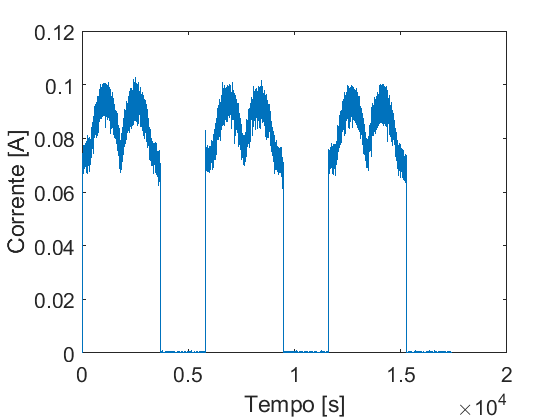
\includegraphics[scale=0.5]{figures/testPanel1Current.png}
\caption{Corrente do Painel 1}
\label{figura_teste_corrente_painel1}
\end{center}
\end{figure}

\begin{figure}[!htpb]
\begin{center}
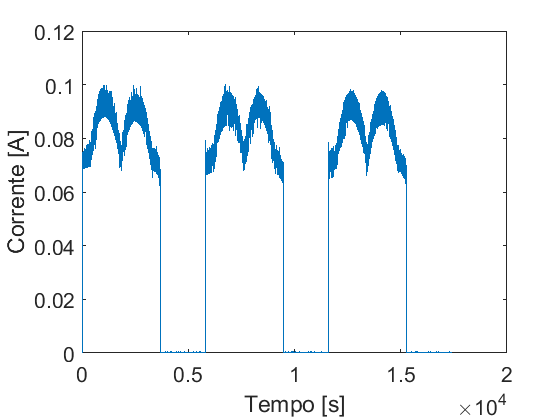
\includegraphics[scale=0.5]{figures/testPanel2Current.png}
\caption{Corrente do Painel 2}
\label{figura_teste_corrente_painel2}
\end{center}
\end{figure}

\begin{figure}[!htpb]
\begin{center}
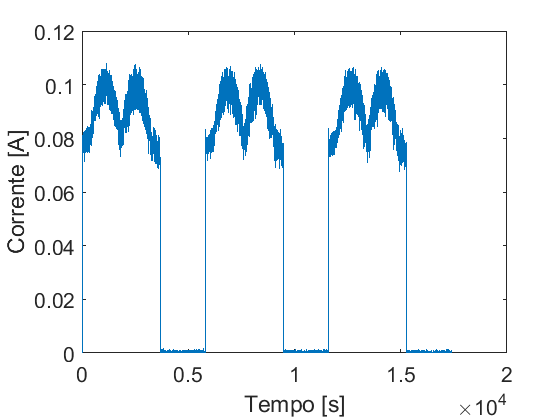
\includegraphics[scale=0.5]{figures/testPanel3Current.png}
\caption{Corrente do Painel 3}
\label{figura_teste_corrente_painel3}
\end{center}
\end{figure}

Da mesma forma, vemos nas figuras \ref{figura_teste_potencia_painel1}, \ref{figura_teste_potencia_painel2} e \ref{figura_teste_potencia_painel3} que a soma das potências ficou próxima ao valor simulado. Inclusive, a figura \ref{figura_potencia_comaracao} apresenta a soma das potências do teste no mesmo gráfico com a potência simulada, e vemos que o resultado está próximo.

\begin{figure}[!htpb]
\begin{center}
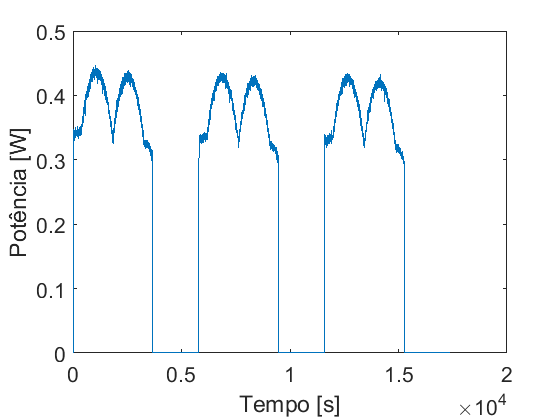
\includegraphics[scale=0.5]{figures/testPanel1Power.png}
\caption{Potência do Painel 1}
\label{figura_teste_potencia_painel1}
\end{center}
\end{figure}

\begin{figure}[!htpb]
\begin{center}
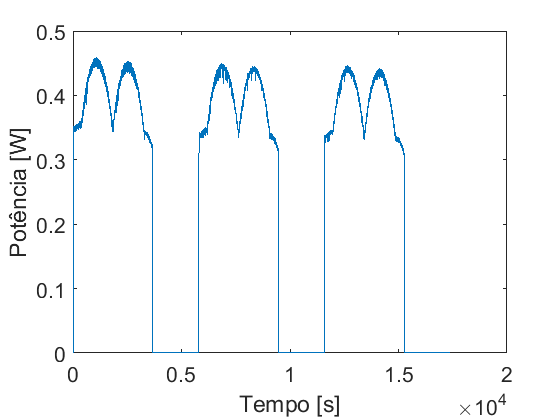
\includegraphics[scale=0.5]{figures/testPanel2Power.png}
\caption{Potência do Painel 2}
\label{figura_teste_potencia_painel2}
\end{center}
\end{figure}

\begin{figure}[!htpb]
\begin{center}
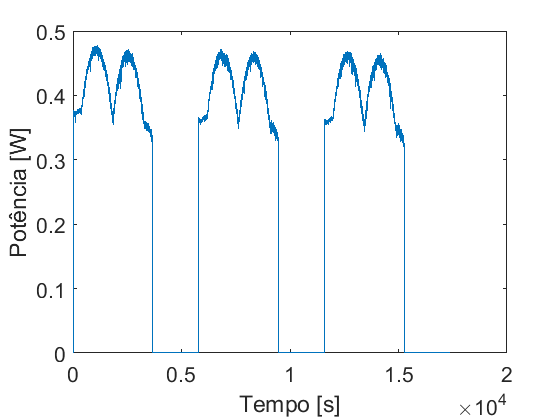
\includegraphics[scale=0.5]{figures/testPanel3Power.png}
\caption{Potência do Painel 3}
\label{figura_teste_potencia_painel3}
\end{center}
\end{figure}

\begin{figure}[!htpb]
\begin{center}
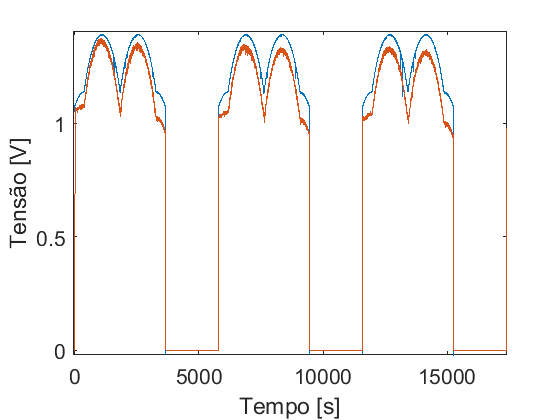
\includegraphics[scale=0.5]{figures/powerComparison.png}
\caption{Comparação das Potências}
\label{figura_potencia_comaracao}
\end{center}
\end{figure}

Nas figuras \ref{figura_teste_tensao_painel1}, \ref{figura_teste_tensao_painel2} e \ref{figura_teste_tensao_painel3} podemos ver o \gls{mppt} em ação realizando o controle da tensão.

\begin{figure}[!htpb]
\begin{center}
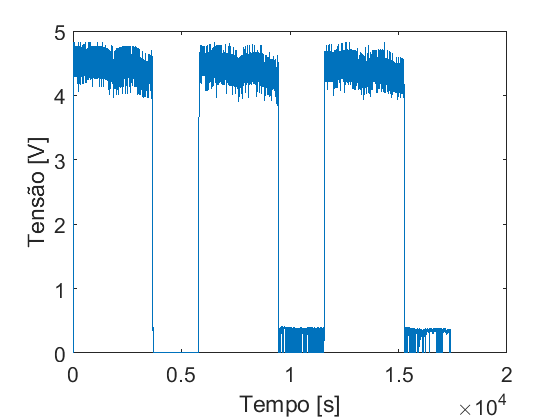
\includegraphics[scale=0.5]{figures/testPanel1Voltage.png}
\caption{Tensão do Painel 1}
\label{figura_teste_tensao_painel1}
\end{center}
\end{figure}

\begin{figure}[!htpb]
\begin{center}
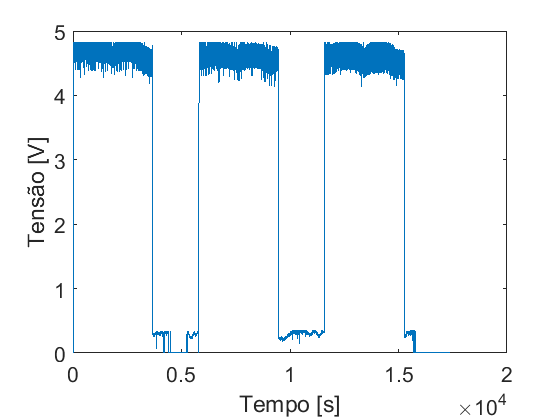
\includegraphics[scale=0.5]{figures/testPanel2Voltage.png}
\caption{Tensão do Painel 2}
\label{figura_teste_tensao_painel2}
\end{center}
\end{figure}

\begin{figure}[!htpb]
\begin{center}
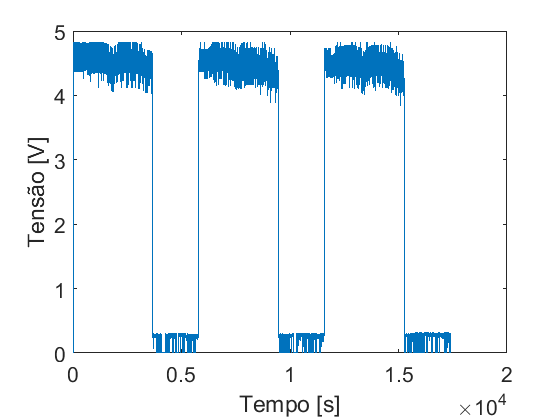
\includegraphics[scale=0.5]{figures/testPanel3Voltage.png}
\caption{Tensão do Painel 3}
\label{figura_teste_tensao_painel3}
\end{center}
\end{figure}

Por fim temos as tensões das baterias 1 e 2 (figuras \ref{figura_teste_tensao_bat1} e \ref{figura_teste_tensao_bat2}). Vemos que este resultado teve uma mudança significativa em relação a simulação, sendo que a tensão diminuiu mais no teste real. Isso se deu por causa da ausência de perdas na simulação, principalmente no conversor \textit{Boost} que conecta os painéis solares às baterias e também pela diferença nas potências de entrada da simulação e a entrada real. Desta forma, a quantidade de energia que entra no sistema durante a região iluminada da curva de irradiância é menor e, consequentemente, a energia disponível durante o período de eclipse é menor.

\begin{figure}[!htpb]
\begin{center}
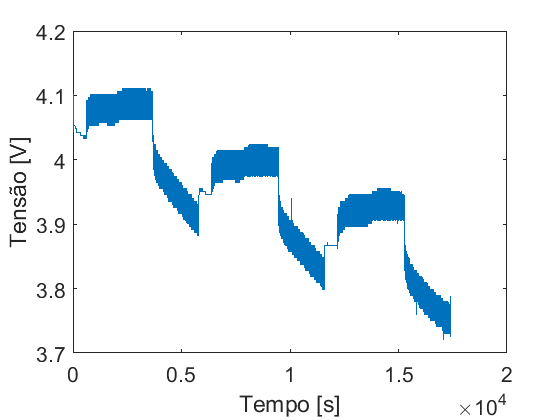
\includegraphics[scale=0.5]{figures/testBat1Voltage.png}
\caption{Tensão da Bateria 1}
\label{figura_teste_tensao_bat1}
\end{center}
\end{figure}

\begin{figure}[!htpb]
\begin{center}
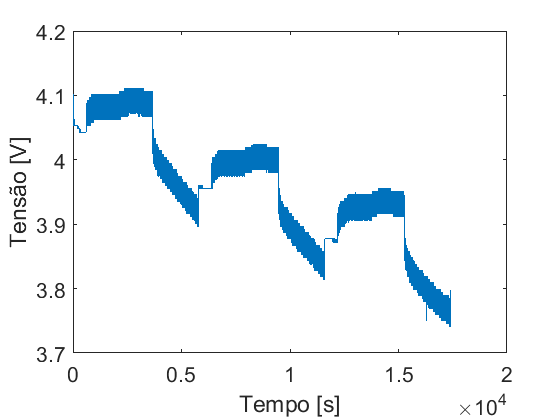
\includegraphics[scale=0.5]{figures/testBat2Voltage.png}
\caption{Tensão da Bateria 2}
\label{figura_teste_tensao_bat2}
\end{center}
\end{figure}

Para quantificar a diferença de energia entre as cargas vamos integrar a potência dos painéis e a potência nas baterias, onde o sinal negativo indica que a potência está saindo das baterias.

\begin{equation}
\int_{0}^{17390} P_{pv}(t) dt = \SI{13.77}{\kilo\joule}
\end{equation} 

\begin{equation}
\int_{0}^{17390} P_{bat}(t) dt = \SI{-22.86}{\kilo\joule}
\end{equation}

Em primeira análise a energia consumida pelas cargas é maior do que a entrege pelos painéis, porém a irradiância utilizada nos testes não corresponde a irradiância incidente do sol no espaço. Na verdade o valor utilizado foi o máximo possível obtido com a bancada disponível, porém representa apenas aproximadamente metade do valor real (\SI{1367}{\watt\per\square\metre} de pico), o que já tornaria a entrada de energia maior do que o consumo. Portanto, pode-se concluir que o sistema está projetado de forma adequada para atender as cargas solicitadas.